\chapter{Domain decomposition}
\label{chap: dom_decomp}
In this chapter two possible domain decomposition algorithms will be presented: the slab decomposition and the pencil decomposition. Sections \ref{sec: slab} and \ref{sec: pencil} will be dedicated to the detailed explanation of these parallelization strategies, focusing also on their strengths and limitations. Section \ref{sec: benchmark} will present a benchmark between these strategies, together with some scalability results.

\section{Slab decomposition}
\label{sec: slab}
The slab decomposition is the simpler case of domain decomposition presented here. The domain is divided in so called slabs which contain all the data in two directions and only a part of the data in the remaining direction.\\
Since here a pseudospectral method is used and when performing transforms each MPI process must hold all the data in the transform direction, during the passage from physical to modal space (and backwards) MPI processes must exchange data. 
\begin{figure}[h!]
\centering
\begin{subfigure}{0.45\textwidth}
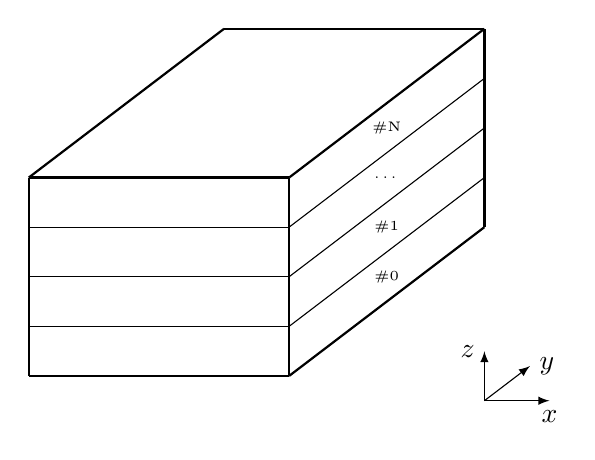
\begin{tikzpicture}[scale=1.4]
\begin{scope}[x={0 250},y={0 200}]
%        %% next four lines will help you to locate the point needed by forming a grid. comment these four lines in the final picture.↓
%        \draw[help lines,xstep=.1,ystep=.1] (0,0) grid (1,1);
%        \draw[help lines,xstep=.05,ystep=.05] (0,0) grid (1,1);
%        \foreach \x in {0,1,...,9} { \node [anchor=north] at (\x/10,0) {0.\x}; }
%        \foreach \y in {0,1,...,9} { \node [anchor=east] at (0,\y/10) {0.\y};}
%        %% upto here↑

% domain
\draw[thick] (0.1,0.1) -- (0.5,0.1);
\draw[thick] (0.1,0.1) -- (0.1,0.5);
\draw[thick] (0.1,0.5) -- (0.5,0.5);
\draw[thick] (0.5,0.1) -- (0.5,0.5);
\draw[thick] (0.5,0.1) -- (0.8,0.4);
\draw[thick] (0.5,0.5) -- (0.8,0.8);
\draw[thick] (0.8,0.4) -- (0.8,0.8);
\draw[thick] (0.1,0.5) -- (0.4,0.8);
\draw[thick] (0.4,0.8) -- (0.8,0.8);

% axis
\draw[-latex] (0.8,0.05) -- (0.9,0.05)node[anchor=north]{$x$};
\draw[-latex] (0.8,0.05) -- (0.8,0.15)node[anchor=east]{$z$};
\draw[-latex] (0.8,0.05) -- (0.87,0.12)node[anchor=west]{$y$};

% decomposition
\draw (0.1,0.2) -- (0.5,0.2);
\draw (0.1,0.3) -- (0.5,0.3);
\draw (0.1,0.4) -- (0.5,0.4);
\draw (0.8,0.5) -- (0.5,0.2);
\draw (0.8,0.6) -- (0.5,0.3);
\draw (0.8,0.7) -- (0.5,0.4);

% ranks
\draw (0.65,0.3)node[rotate=0]{\tiny{\#0}};
\draw (0.65,0.4)node[rotate=0]{\tiny{\#1}};
\draw (0.65,0.5)node[rotate=0]{\tiny{\dots}};
\draw (0.65,0.6)node[rotate=0]{\tiny{\#N}};

\end{scope}
\end{tikzpicture}

\subcaption{Slab decomposition, physical space}
\end{subfigure}%
\hspace{0.5cm}
\begin{subfigure}{0.45\textwidth}
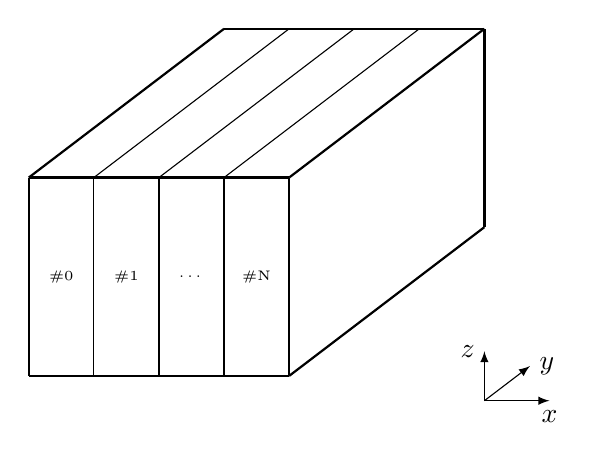
\begin{tikzpicture}[scale=1.4]
\begin{scope}[x={0 250},y={0 200}]
%        %% next four lines will help you to locate the point needed by forming a grid. comment these four lines in the final picture.↓
%        \draw[help lines,xstep=.1,ystep=.1] (0,0) grid (1,1);
%        \draw[help lines,xstep=.05,ystep=.05] (0,0) grid (1,1);
%        \foreach \x in {0,1,...,9} { \node [anchor=north] at (\x/10,0) {0.\x}; }
%        \foreach \y in {0,1,...,9} { \node [anchor=east] at (0,\y/10) {0.\y};}
%        %% upto here↑

% domain
\draw[thick] (0.1,0.1) -- (0.5,0.1);
\draw[thick] (0.1,0.1) -- (0.1,0.5);
\draw[thick] (0.1,0.5) -- (0.5,0.5);
\draw[thick] (0.5,0.1) -- (0.5,0.5);
\draw[thick] (0.5,0.1) -- (0.8,0.4);
\draw[thick] (0.5,0.5) -- (0.8,0.8);
\draw[thick] (0.8,0.4) -- (0.8,0.8);
\draw[thick] (0.1,0.5) -- (0.4,0.8);
\draw[thick] (0.4,0.8) -- (0.8,0.8);

% axis
\draw[-latex] (0.8,0.05) -- (0.9,0.05)node[anchor=north]{$x$};
\draw[-latex] (0.8,0.05) -- (0.8,0.15)node[anchor=east]{$z$};
\draw[-latex] (0.8,0.05) -- (0.87,0.12)node[anchor=west]{$y$};

% decomposition
\draw (0.2,0.1) -- (0.2,0.5);
\draw (0.3,0.1) -- (0.3,0.5);
\draw (0.4,0.1) -- (0.4,0.5);
\draw (0.5,0.8) -- (0.2,0.5);
\draw (0.6,0.8) -- (0.3,0.5);
\draw (0.7,0.8) -- (0.4,0.5);

% ranks
\draw (0.15,0.3)node[rotate=0]{\tiny{\#0}};
\draw (0.25,0.3)node[rotate=0]{\tiny{\#1}};
\draw (0.35,0.3)node[rotate=0]{\tiny{\dots}};
\draw (0.45,0.3)node[rotate=0]{\tiny{\#N}};

\end{scope}
\end{tikzpicture}

\subcaption{Slab decomposition, modal space}
\end{subfigure}
\caption{Slab decomposition, MPI processes numbering}
\label{fig: slab}
\end{figure}
As shown in Figure \ref{fig: slab} in physical space each MPI process holds all the data in a $x-y$ plane and only a part of data in the $z$ direction, while in modal space each MPI process hold all data in a $y-z$ plane and only a part of data in the $x$ direction.\\
When in physical space 1D Fourier transforms are performed in the $x$ and $y$ directions; then all MPI processes exchange data to transpose the slabs from the $x-y$ plane to the $y-z$ plane and a 1D Chebyshev transform is performed in the wall-normal direction. At this point the data are in modal space.\\
The slab decomposition requires one series of MPI communication among all MPI processes for each passagge for physical [modal] space to modal [physical] space. The way the domain is divided among all processes restricts the maximum number of MPI processes that can actually be used: using a $N^3$ domain limits the maximum number of processes to roughly $N$. In fact each MPI process must hold at least a plane of data ($N\times N\times 1$). This limit thus depends on the choice of the grid.\\
Using the slab decomposition method allows to reduce the number of MPI communications but poses a strong limit on the maximum number of MPI processes.

\section{Pencil decomposition}
\label{sec: pencil}
The pencil decomposition strongly increases the limit on the maximum number of MPI processes that can be used at the cost of an increased number of MPI communication. With this strategy each MPI process holds all the data in one direction and part of the data in the other two directions.
\begin{figure}[h!]
\centering
\begin{subfigure}{0.45\textwidth}
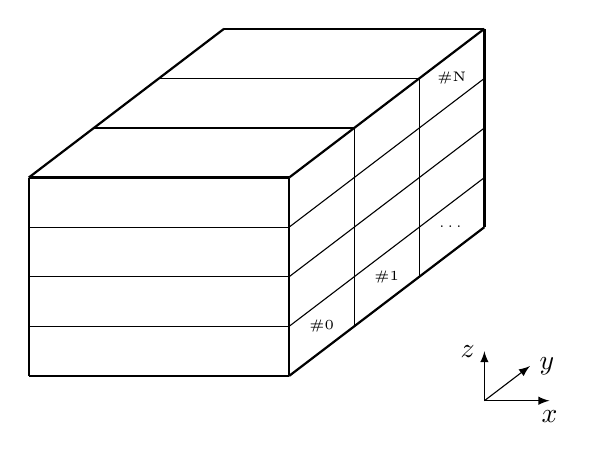
\begin{tikzpicture}[scale=1.4]
\begin{scope}[x={0 250},y={0 200}]
%        %% next four lines will help you to locate the point needed by forming a grid. comment these four lines in the final picture.↓
%        \draw[help lines,xstep=.1,ystep=.1] (0,0) grid (1,1);
%        \draw[help lines,xstep=.05,ystep=.05] (0,0) grid (1,1);
%        \foreach \x in {0,1,...,9} { \node [anchor=north] at (\x/10,0) {0.\x}; }
%        \foreach \y in {0,1,...,9} { \node [anchor=east] at (0,\y/10) {0.\y};}
%        %% upto here↑

% domain
\draw[thick] (0.1,0.1) -- (0.5,0.1);
\draw[thick] (0.1,0.1) -- (0.1,0.5);
\draw[thick] (0.1,0.5) -- (0.5,0.5);
\draw[thick] (0.5,0.1) -- (0.5,0.5);
\draw[thick] (0.5,0.1) -- (0.8,0.4);
\draw[thick] (0.5,0.5) -- (0.8,0.8);
\draw[thick] (0.8,0.4) -- (0.8,0.8);
\draw[thick] (0.1,0.5) -- (0.4,0.8);
\draw[thick] (0.4,0.8) -- (0.8,0.8);

% axis
\draw[-latex] (0.8,0.05) -- (0.9,0.05)node[anchor=north]{$x$};
\draw[-latex] (0.8,0.05) -- (0.8,0.15)node[anchor=east]{$z$};
\draw[-latex] (0.8,0.05) -- (0.87,0.12)node[anchor=west]{$y$};

% decomposition
\draw (0.1,0.2) -- (0.5,0.2);
\draw (0.1,0.3) -- (0.5,0.3);
\draw (0.1,0.4) -- (0.5,0.4);
\draw (0.8,0.5) -- (0.5,0.2);
\draw (0.8,0.6) -- (0.5,0.3);
\draw (0.8,0.7) -- (0.5,0.4);
\draw (0.6,0.2) -- (0.6,0.6);
\draw (0.7,0.3) -- (0.7,0.7);
\draw (0.2,0.6) -- (0.6,0.6);
\draw(0.3,0.7) -- (0.7,0.7);

% ranks
\draw (0.55,0.2)node[rotate=0]{\tiny{\#0}};
\draw (0.65,0.3)node[rotate=0]{\tiny{\#1}};
\draw (0.75,0.4)node[rotate=0]{\tiny{\dots}};
\draw (0.75,0.7)node[rotate=0]{\tiny{\#N}};

\end{scope}
\end{tikzpicture}

\subcaption{Pencil decomposition, physical space}
\end{subfigure}%
\hspace{0.5cm}
\begin{subfigure}{0.45\textwidth}
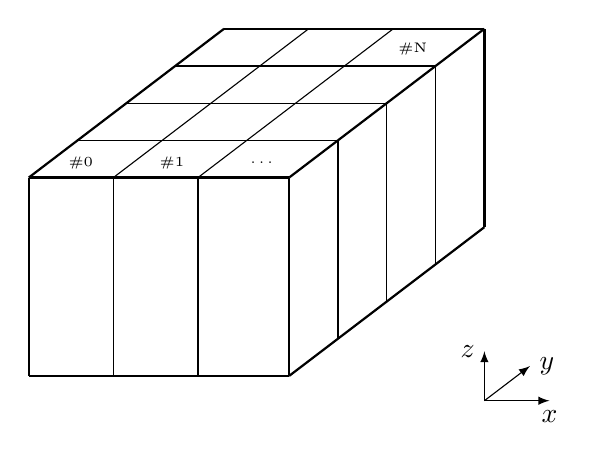
\begin{tikzpicture}[scale=1.4]
\begin{scope}[x={0 250},y={0 200}]
%        %% next four lines will help you to locate the point needed by forming a grid. comment these four lines in the final picture.↓
%        \draw[help lines,xstep=.1,ystep=.1] (0,0) grid (1,1);
%        \draw[help lines,xstep=.05,ystep=.05] (0,0) grid (1,1);
%        \foreach \x in {0,1,...,9} { \node [anchor=north] at (\x/10,0) {0.\x}; }
%        \foreach \y in {0,1,...,9} { \node [anchor=east] at (0,\y/10) {0.\y};}
%        %% upto here↑

% domain
\draw[thick] (0.1,0.1) -- (0.5,0.1);
\draw[thick] (0.1,0.1) -- (0.1,0.5);
\draw[thick] (0.1,0.5) -- (0.5,0.5);
\draw[thick] (0.5,0.1) -- (0.5,0.5);
\draw[thick] (0.5,0.1) -- (0.8,0.4);
\draw[thick] (0.5,0.5) -- (0.8,0.8);
\draw[thick] (0.8,0.4) -- (0.8,0.8);
\draw[thick] (0.1,0.5) -- (0.4,0.8);
\draw[thick] (0.4,0.8) -- (0.8,0.8);

% axis
\draw[-latex] (0.8,0.05) -- (0.9,0.05)node[anchor=north]{$x$};
\draw[-latex] (0.8,0.05) -- (0.8,0.15)node[anchor=east]{$z$};
\draw[-latex] (0.8,0.05) -- (0.87,0.12)node[anchor=west]{$y$};

% decomposition
\draw (0.23,0.1) -- (0.23,0.5);
\draw (0.36,0.1) -- (0.36,0.5);
\draw (0.53,0.8) -- (0.23,0.5);
\draw (0.66,0.8) -- (0.36,0.5);
\draw (0.575,0.175) -- (0.575,0.575);
\draw (0.65,0.25) -- (0.65,0.65);
\draw(0.725,0.325) -- (0.725,0.725);
\draw (0.175,0.575) -- (0.575,0.575);
\draw (0.25,0.65) -- (0.65,0.65);
\draw(0.325,0.725) -- (0.725,0.725);

% ranks
\draw (0.18,0.53)node[rotate=0]{\tiny{\#0}};
\draw (0.32,0.53)node[rotate=0]{\tiny{\#1}};
\draw (0.46,0.53)node[rotate=0]{\tiny{\dots}};
\draw (0.69,0.76)node[rotate=0]{\tiny{\#N}};


\end{scope}
\end{tikzpicture}

\subcaption{Pencil decomposition, modal space}
\end{subfigure}
\caption{Pencil decomposition, MPI processes numbering}
\label{fig: pencil}
\end{figure}
When passing from physical space to modal space, according to Figure \ref{fig: pencil}, first a 1D Fourier transform is performed in the $x$ direction, then there is a series of MPI communications such that each rank, after that, holds all the data in the $y$ direction. Then, a 1D Fourier transform is performed in the $y$ direction; again there is a series of MPI communication such that each MPI process then holds all data in the $z$ direction. Finally a 1D Chebyshev transform is performed in the $z$ direction. In order to pass from modal space to physical space, all the previous steps must be done in reverse order.\\
The pencil decomposition strategy thus strongly increases the maximum number of MPI processes that can be used: a domain with $N^3$ point can be parallelized up to roughly $N^2$ MPI processes (each MPI process hold $N\times1\times1$ points with the highest number of MPI processes). The cost for this increasing in the maximum number of MPI processes is a higher number of MPI communication: now there are two series of MPI communications.\\
In the pencil domain decomposition case a doubly periodic Cartesian topology can be used to find out in a much easier way which are the MPI processes involved in the communications. For example, in the first MPI communication series only the MPI processes in the same $x-y$ plane exchange data, while in the second MPI communication series only the MPI processes belonging to the same $y-z$ plane exchange data.


\section{Domain decomposition strategies benchmark}
\label{sec: benchmark}
Some test cases were run on the Marconi A1 Broadwell partition to verify the scalability of the code. The Marconi A1 partition machine has 1\,512 nodes, each one with 36 cores/node, for a total of 54\,432 cores. Each node is made up of two socket; each one is an Intel Xeon E5-2697 v4 @2.3 GHz. The total amount of RAM memory available per node is 128 GB/node, but it is suggested to use up to $\sim$120 GB/node.\\
Two kind of scalability tests were run: a strong scalability analysis and a weak scalability one. In the strong scalability case the overall domain size is kept constant, while the number of MPI processes is increased. As the number of MPI processes increases, the load on each core is reduced (lower number of points per core). In the weak scalability case the load (number of points per core) is kept constant while the overall number of points is increased according to the increase in the number of MPI processes.\\
\begin{figure}[h!]
\centering
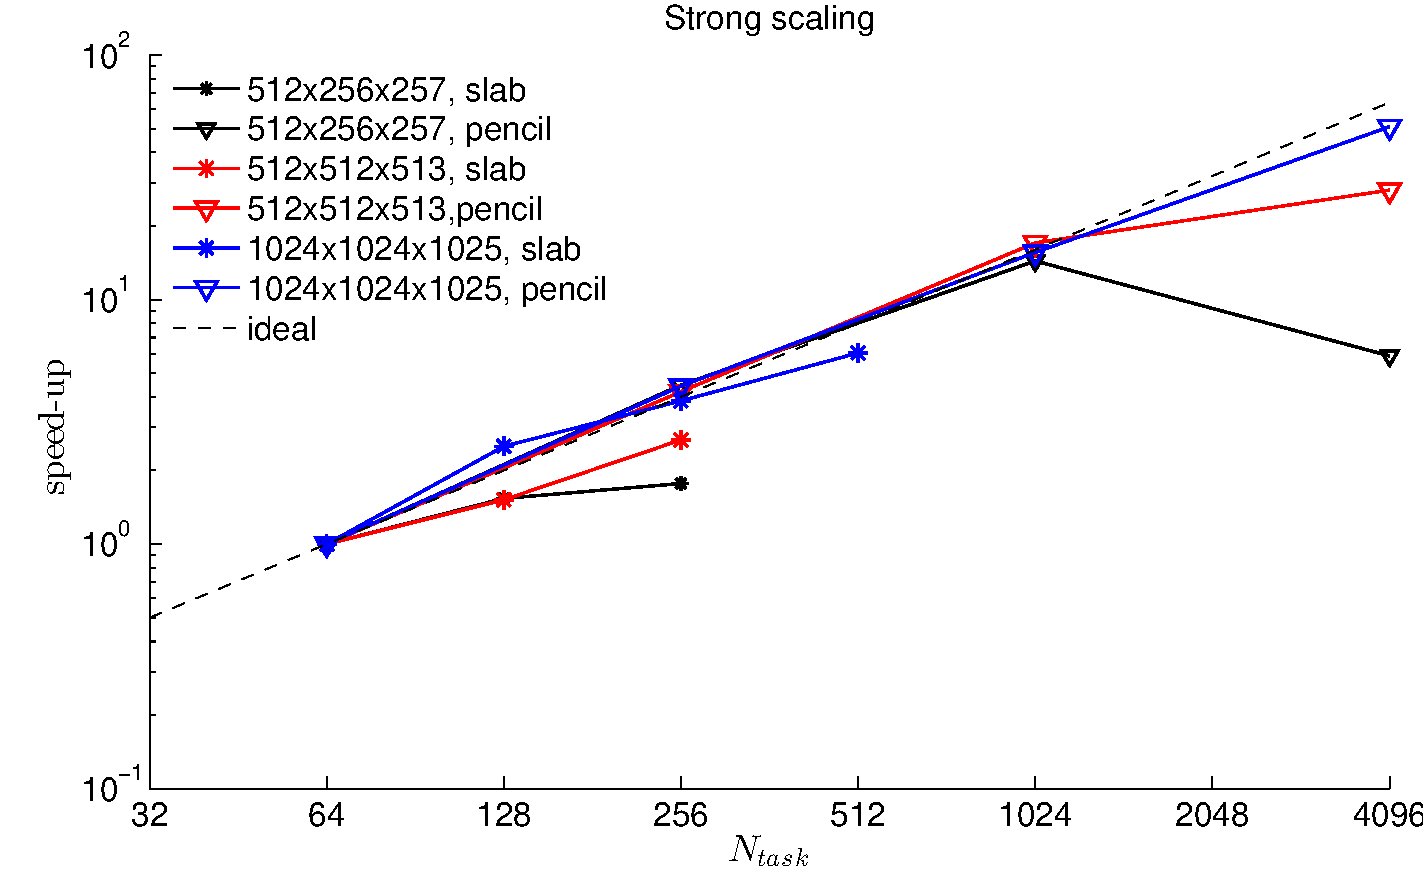
\includegraphics[width=0.9\textwidth]{strong_s_64}
\caption{Strong scalability}
\label{fig: strong_s}
\end{figure}
For the strong scalability case three different grids were tested both for slab and pencil domain decomposition: $512\times256\times257$, $512\times512\times513$ and $1024\times1024\times1025$. As commonly found in literature the speed-up obtained is normalized by the speed-up obtained on the lowest number of MPI processes used; in this case the lowest number was 64 MPI processes. The ideal behaviour is linear in the total number of MPI processes; as can be seen from Figure \ref{fig: strong_s} the slab decomposition runs deviate quite early from the ideal case, while the pencil cases keep an optimal speed-up at least up to 1\,024 MPI processes. At this point only the larger grid does not show worsening in the performance, while the smaller grids show a larger deviation from the ideal case. Due to the limit on the maximum number of cores  that can be requested on the Marconi A1 partition (around 6\,000), we could not verify the scalability on a higher number of MPI processes.\\
\begin{table}[H]
\centering
\caption{Strong scaling speed-up calculated with respect to 64 MPI processes case}
\begin{tabular}{c|c|c|c|c|c}
$N_{y,cpu}$ & $N_{z,cpu}$ & grid & time per time step [s] & speed-up &ideal speed-up\\[1.5ex]
1 & 64 & $512\times256\times257$&1.22 & 1& 1\\
1 & 128 & $512\times256\times257$& 0.79 &1.54& 2\\
1 &256& $512\times256\times257$& 0.69 & 1.77 &4\\
\hline
8& 8& $512\times256\times257$& 1.44  & 1 &1\\
16& 16 & $512\times256\times257$& 0.32 & 4.5& 4 \\
32 &32 & $512\times256\times257$& 0.10 & 14.4 &16 \\
64 &64 & $512\times256\times257$& 0.25 & 5.76 &64\\
\hline\hline
1& 64 & $512\times512\times513$& 4.82  & 1 &1\\
1& 128& $512\times512\times513$& 3.18  & 1.52 &2 \\
1 &256& $512\times512\times513$& 1.81 & 2.66 &4\\
\hline
8& 8 & $512\times512\times513$& 6.64 &  1 &1\\
16& 16 & $512\times512\times513$&1.58 & 4.20 &4\\
32 &32 & $512\times512\times513$&0.39& 17.03 &16\\
64 &64 & $512\times512\times513$&0.24 &  27.67 &64\\
\hline\hline
1& 64 & $1024\times1024\times1025$& 55.72 &1  &1 \\
1& 128& $1024\times1024\times1025$& 22.20 & 2.51 &2\\
1 &256& $1024\times1024\times1025$& 14.46 &3.85 &4\\
1 &512 & $1024\times1024\times1025$&9.20 & 6.06 &8\\
\hline
8& 8 & $1024\times1024\times1025$&62.40 & 1 &1\\
16& 16& $1024\times1024\times1025$& 14.10 & 4.43 &4\\
32 &32& $1024\times1024\times1025$& 4.00 &  15.6 &16\\
64 &64& $1024\times1024\times1025$& 1.23 & 50.73  &64\\
\end{tabular}
\end{table}
\begin{figure}[h!]
\centering
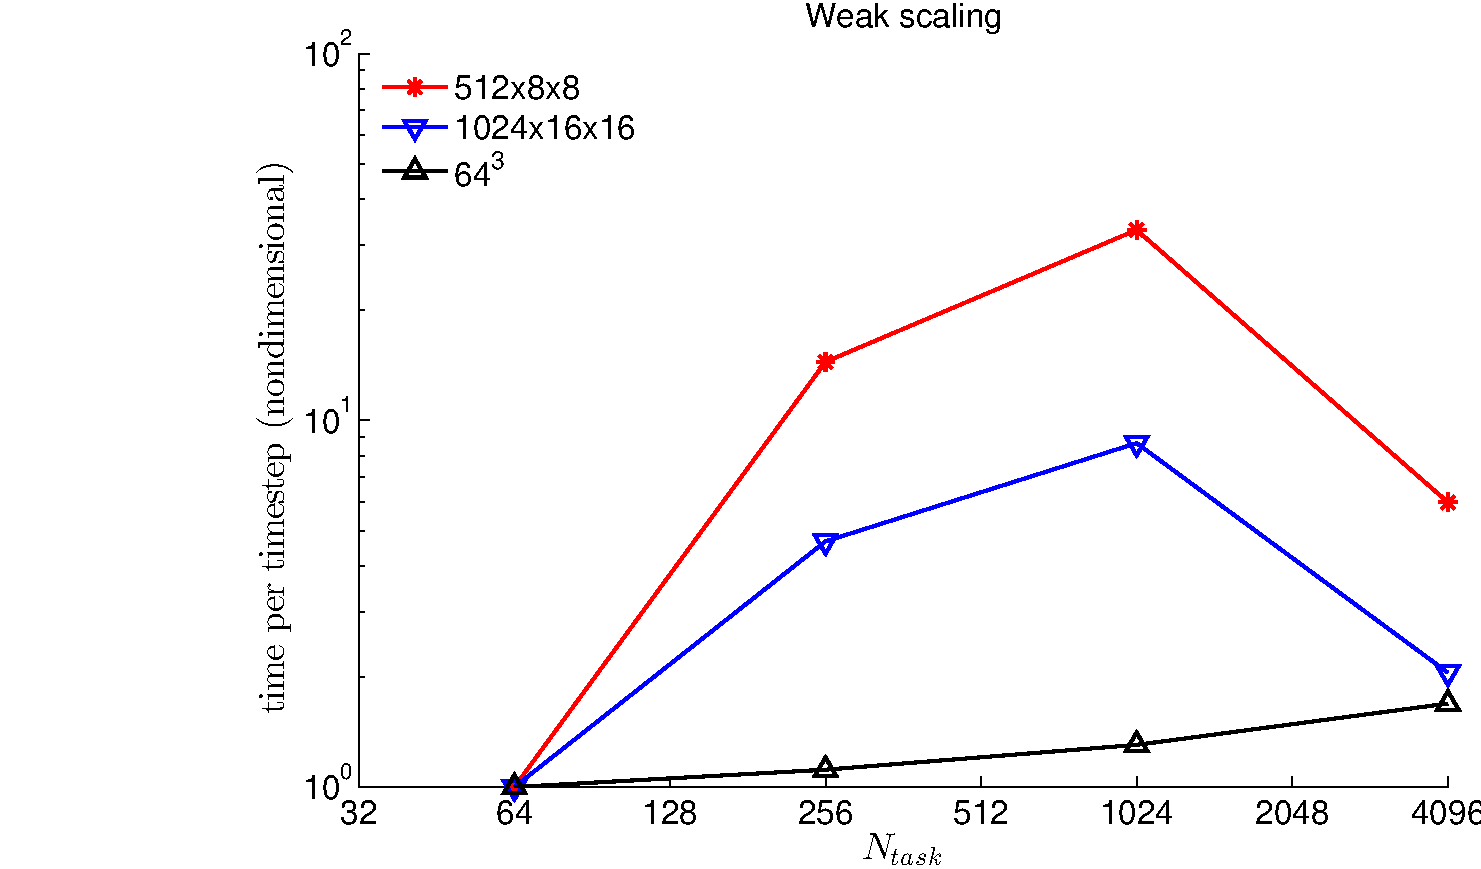
\includegraphics[width=0.9\textwidth]{weak_s_64}
\caption{Weak scalability}
\end{figure}
For the weak scalability case three different runs were run: in the first two cases denoted by $512\times8\times8$ and $1024\times16\times16$ the aspect ratio of the arrays was kept constant as the number of MPI processes increased. In the other case, denoted by $64^3$ only the total number of points per MPI process was kept constant. This allowed for a better data layout in memory, which gave much better results, only matched by the others two cases when the global grid approached a unitary aspect ratio in the three dimensions.
\begin{table}[H]
\centering
\caption{Weak scaling time per time step normalized with respect to 64 MPI processes case}
\begin{tabular}{c|c|c|c|c|c}
$N_{y,cpu}$ & $N_{z,cpu}$& load/core & grid & $t/t_{\textnormal{step}}$ [s] &$t/t_{\textnormal{step}}$ normalized\\[1.5ex]
8& 8 & $512\times8\times8$  &$512\times64\times65$ &  0.06 & 1\\
16 &16&$512\times8\times8$  & $512\times128\times129$& 0.81 & 14.46\\
32 &32&$512\times8\times8$  & $512\times256\times257$& 1.85 & 33.04\\
64 &64 &$512\times8\times8$  &$512\times512\times513$ & 0.34 & 6.07 \\
\hline
8& 8&$1024\times16\times16$  & $1024\times128\times129$ &0.54 &1 \\
16& 16& $1024\times16\times16$  & $1024\times256\times257$ &2.50 & 4.66\\
32 &32 &$1024\times16\times16$  & $1024\times512\times513$ &4.64 & 8.66\\
64 &64 &$1024\times16\times16$  & $1024\times1024\times1025$ &1.10 & 2.05\\
\hline
8& 8 & $64^3$& $256\times256\times257$ & 0.65& 1\\
16& 16&$64^3$&$512\times512\times257$ & 0.73 &1.12 \\
32& 32 &$64^3$&$512\times512\times1025$ &0.85 & 1.30 \\
64& 64 &$64^3$&$1024\times1024\times1025$ &1.10 &1.69 \\ 
\end{tabular}
\end{table}








